\documentclass{CUP-JNL-DTM}%


%%%% Packages
\usepackage{graphicx}
\usepackage{multicol,multirow}
\usepackage{amsmath,amssymb,amsfonts}
\usepackage{mathrsfs}
\usepackage{amsthm}
\usepackage{rotating}
\usepackage{appendix}
\usepackage[numbers]{natbib}
\usepackage{ifpdf}
\usepackage[T1]{fontenc}
\usepackage{newtxtext}
\usepackage{newtxmath}
\usepackage{textcomp}
\usepackage{xcolor}
\usepackage{lipsum}
\usepackage[colorlinks,allcolors=blue]{hyperref}

\newtheorem{theorem}{Theorem}[section]
\newtheorem{lemma}[theorem]{Lemma}
\theoremstyle{definition}
\newtheorem{remark}[theorem]{Remark}
\newtheorem{example}[theorem]{Example}
\numberwithin{equation}{section}


\jname{Environmental Data Science}
\articletype{DATA PAPER}
%\artid{20}
\jyear{YEAR}
%\jvol{4}
%\jissue{1}
%\raggedbottom


\begin{document}

\begin{Frontmatter}

\title[Article Title]{Data-driven Attributing of Climate Events with \\Climate Index Collection based on Model Data (CICMoD)}

\author[1,3]{Marco Landt-Hayen}\orcid{0000-0003-3606-7760}
\author[1]{Willi Rath}\orcid{0000-0003-1951-8494}
\author[1]{Sebastian Wahl}\orcid{0000-0002-1360-5776}
\author[1]{Nils Niebaum}
\author[2]{Martin Claus}\orcid{0000-0002-7525-5134}

\authormark{Landt-Hayen \textit{et al}.}

\address[1]{\orgdiv{Ocean Circulation and Climate Dynamics}, \orgname{GEOMAR Helmholtz Centre for Ocean Research}, \orgaddress{\city{Kiel}, \country{Germany}}} 

\address[2]{\orgname{Christian-Albrechts-Universität zu Kiel and GEOMAR Helmholtz Centre for Ocean Research}, \orgaddress{\city{Kiel},  \country{Germany}}}

\address[3]{Corresponding author. E-mail: mlandt-hayen@geomar.de}

\keywords{Time Series Forecasting, Artificial Neural Networks, Explainable AI, Interpretable ML, Data Mining}

\keywords[MSC Codes]{\codes[Primary]{CODE1}; \codes[Secondary]{CODE2, CODE3}}

\abstract{Machine learning (ML) and in particular artificial neural networks (ANNs) push state-of-the-art solutions for many hard problems e.g., image classification, speech recognition or time series forecasting. In the domain of climate science, ANNs have good prospects to identify causally linked modes of climate variability as key to understand the climate system and to improve the predictive skills of forecast systems. The data science community provides standard data sets for many applications. However, there exists no consistent and comprehensive collection of climate indices covering Earth System dynamics. To attribute climate events in a data-driven way with ANNs, we need sufficient training data, which is often limited for real world measurements. With only short time series available, it is difficult to train ML models and in particular ANNs, that generalize well. Here, we use control runs from Earth System Models over 1,000 years and derive a consistent collection of climate indices. As exemplary applications, we use the data set to predict rainfall in the African Sahel region and El Ni\~{n}o Southern Oscillation with various ML models. But these models tend to produce black box results that are difficult to interpret even by ML experts. We argue that this new data set allows to thoroughly explore techniques from the domain of explainable artificial intelligence to have trustworthy models, that are accepted by domain scientists. The aim is to build a bridge between the computer science and data science community on the one hand and researchers and practitioners from the domain of climate science.}

\end{Frontmatter}

\section*{Impact Statement}
Machine learning (ML) models learn from data. To compare and improve ML methods and models, data scientists need standard data sets as benchmark. There exist many standard data sets, like a collection of handwritten digits or images. Our contribution is, to add a consistent and comprehensive collection of climate indices as new data set. This collection can be used to train ML models to understand the climate system with its complex short- and long-term variabilities and to predict climate events. Additionally, the aim is to understand how the models learn and how they come to their conclusion, which is referred to as explainable artificial intelligence. Only if we understand the models in great detail, we gain trust in the results.

\section{Introduction \label{sec:Introduction}}

To apply and compare machine learning (ML) methods and models, there exist standard data sets as benchmark. Among these data sets, we find e.g. a collection of handwritten digits provided by the National Institute of Standards and Technology, referred to as MNIST data set \cite{Lecun1998}. Other data sets contain images, like the CIFAR-10 data set from Canadian Institute for Advanced Research, introduced by Krizhevsky \cite{Krizhevsky2009}. Or so-called Fisherfaces, as a collection of human faces in different pose \cite{Belhumeur1997}. These data sets are mostly suitable for classification algorithms. Famous data sets for pattern recognition and clustering applications are e.g. Iris or Wine data sets, provided by UCI Machine Learning Repository \cite{Murphy1994}, containing attributes for various species of the Iris plant and results of a chemical analysis of wines, respectively. Furthermore, the data science community also provides standard time series collections, like the RAE data set that contains energy consumption for various household appliances as time series \cite{Makonin2018}. 

Here, we are interested in describing the underlying dynamics of the Earth System. Real world data is limited to observable features that can be measured in a comprehensive way or that can be reconstructed from sparse measurements. Examples are sea surface temperature (SST), sea level pressure (SLP), sea air temperature (SAT) or geopotential height at various pressure levels, e.g. 500 millibar (Z500). Other features have been measured in the past or are continuously measured only for specific regions by permanent stations that are fixed in place or on trajectories of research cruises. This can be precipitation or sea surface salinity (SSS), respectively. Within these features, some of the main dynamics of the Earth system is reflected in form of known climate variabilities, patterns and oscillations, like e.g. Atlantic Multidecadal Oscillation (AMO), Southern Annular Mode (SAM) or El Ni\~{n}o Southern Oscillation (ENSO). ADD citations! The computational effort to model the Earth System can be reduced, when two-dimensional fields are used to derive specific climate indices that capture main processes. ML models are then trained on a set of one-dimensional time series instead of two-dimensional fields of various features.

For instance, ENSO is a complex phenomenon that can be detected as periodic SST fluctuations in the Tropical Pacific [ADD CITATION]. Several indices are defined to compute the current ENSO phase as area-averaged SST anomaly in certain regions. Morrow et al. define Ni\~{n}o 3.4 index from the Ni\~{n}o 3.4 region (5°N–5°S, 120–170°W) which is often used in the context of ENSO. While ENSO is a large scale driver of the climate system, other indices aim to capture regional variability in specific features, like the Sahel precipitation index (SPI). This index measures anomalies of summertime rainfall in the African Sahel region [ADD CITATION: Badr et al]. Climate indices are limited in their temporal extend, since consistent real world measurements started only in recent history or measurements are subject of specific research projects that run over a certain period in time. 

Climate related time series data can be found e.g. on Kaggle, covering heterogeneous features, regions and time scales with different resolution in space and time \cite{https://www.kaggle.com/datasets/sumanthvrao/daily-climate-time-series-data  or https://www.kaggle.com/datasets/shabanamir/enso-data}.

Other important sources: Cite NAOO source for real-world data. And climateguide.org
CHECK Master Thesis of Klaus Reus: Where did he get the data or pre-computed indices from?

Aber letztlich alles nur Stückwerk! 

Our aim is more general. To better understand existing modes of climate variability and to find new relations, we require a consistent and comprehensive collection of climate indices over the longest possible time span, which restricts the use of real world data. Earth System Models (ESMs) aim to model processes of the Earth system in specified temporal and spatial resolution. The flexible Ocean and Climate interface (FOCI) model [ADD CITATION] is an ESM, that... Another example is the Community Earth System Model (CESM) by ... [ADD CITATION]. The quality of model outputs is evaluated on certain control runs. This can e.g. be done by starting an ESM with pre-industrial conditions from the year 1850 and letting the model unfold its dynamics without external forcing over a desired time span. A control run provides several features. Here, we use the output of FOCI and CESM control runs. In particular, we work with SST, SAT, SLP, Z500, SSS and precipitation as two-dimensional fields. From this data, we derive a set of climate indices over 1,000 and 999 years, respectively. The obtained collection of climate indices based on model data (CICMoD) is taken as reduced description of the Earth system in a consistent and comprehensive way. 

ML models can then be trained on this CICMoD data set and various methods can be compared and to set benchmarks. Relations in the climate systems are often characterized as non-linear and non-stationary [ADD CITATIONS from MarDATA Project proposal]. ML models and methods bear good prospects on this kind of problems. Once we find new relationships in the Earth System, these findings need to be confirmed on real world data to separate facts from model artifacts. A better understanding of causally linked modes within our climate system is essential to tackle climate change and attenuate its impacts. 
The CICMoD project also opens the door to exploit and explore techniques from the domain of interpretable ML to enhance the explainability of ML models to obtain trustworthy results.

The rest of this work is structured as follows. In Section \ref{sec:Model_Data} we describe FOCI and CESM models and give meta data for model outputs that are used to define climate indices. An overview of all indices included in the CICMoD data set and details on how the indices are derived from raw ESM outputs are given in Section \ref{sec:Climate_Index_Collection}. In section \ref{sec:Application_Results} we show two exemplary applications and use climate indices from CICMoD data set to predict ENSO and Sahel rainfall, respectively. A detailed discussion of all results and a conclusion is found in Section \ref{sec:Discussion_Conclusion}.

\section{Model Data \label{sec:Model_Data}}

The Community Earth System Model (CESM) and the Flexible Ocean and Climate Infrastructure (FOCI) are both fully-coupled, global climate models that provide state-of-the-art computer simulations of the Earth's past, present, and future climate states.

This dataset contains results from control runs with conditions of year 1850 without additional external forcing for 1000 years and 999 years for FOCI and CESM, respectively.

Describe ESM in general and key ideas of FOCI and CESM in particular. Describe FOCI and CESM control runs, use 1,000 and 999 years, respectively.

FOCI:
Matthes, K., Biastoch, A., Wahl, S., Harlaß, J., Martin, T., Brücher, T., … Park, W. (2020). The Flexible Ocean and Climate Infrastructure Version 1 (FOCI1): Mean State and Variability. Geoscientific Model Development, 13(6), 1–53. https://doi.org/10.5194/gmd-2019-306

"pre-industrial control run under 1850 climate conditions...", years 501 through 1,500.

CESM:
Wait for Sebastian: Either CESM runs are already published, or he will describe data.

Use geopotential height (Z500), sea level pressure (SLP), sea surface temperature (SST), sea surface salinity (SSS), sea air temperature (SAT) and precipitation fields. 
--> State metadata for raw fields:

Introduce file names of raw ESN output fields, as published on Zenodo:
SST-FOCI: bla.end
SLP-FOCI: blup.end
...
SST-CESM: bla.end
...

Then give spatial and temporala resolution and content for each file, called by short name.

In some cases, re-gridding was applied, why and how?
And something was not identical: SAT 2m Höhe? Should be mentioned!

\section{Climate Index Collection \label{sec:Climate_Index_Collection}}

Cluster derived indices according to Z500, SLP, SST, SSS, SAT and precipitation, like in GitHub release overview. Outline recipe with reference. Remarks on normalization and various techniques: Station-based vs. PC-based.

Show pairwise correlation.

\section{Application and Results \label{sec:Application_Results}}

Introduce Sahel rainfall and ENSO problem in more detail. Then show results and give evaluation measures. Only Sahel rainfall with lin Reg and MLP, plus ENSO with CNN and LSTM, on both, FOCI and ENSO for comparison. No xAI techniques. But contingency tables.

\begin{figure}[]
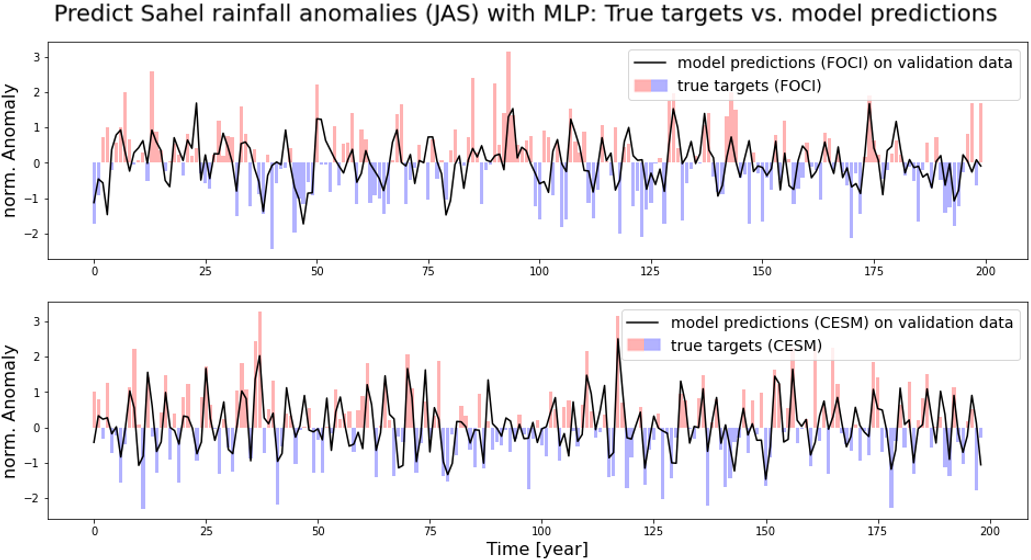
\includegraphics[width=\textwidth]{fig_Sahel_Rainfall_MLP.png}
\caption{Upper part: Composite average SST anomaly patterns for El Ni\~{n}o (left-hand side) and La Ni\~{n}a (right-hand side) events. A black rectangle highlights Ni\~{n}o 3.4 region. Lower part: Exemplary samples for classes 1 (left-hand side) and 2 (right-hand side) of synthetic data.}
\label{fig:Data}
\end{figure}


\section{Discussion and Conclusion \label{sec:Discussion_Conclusion}}

Find higher ENSO frequency in CESM, compared to FOCI. See https://gmd.copernicus.org/articles/13/2533/2020/#Ch1.S4.SS5 in chapter 4.5, where they discuss, how FOCI data reflect ENSO. Periodicity of 2-7 years gives a broad range, covering CESM and FOCI observations.

ESMs are just models and as this, try to approximate Earth System dynamics. Different ESMs have their individual strengths and weaknesses. Advantage, that we have TWO ESM outputs included in CICMoD. Find something new in ONE model, first try to reproduce findings in the OTHER model's data. If yes, try to repeat on real-world data! Working with CICMoD can reveal insights in blind spots by investigating known real world phenomena and comparing with results on indices derived from ESN output. 
Open the door for xAI methods: Create some toolbox as further work! Use data set for Hackathon / competition, push understanding of climate problems in a playfull way!


\begin{Backmatter}

\paragraph{Funding Statement}
This work was supported by the Helmholtz School for Marine Data Science (MarDATA) funded by the Helmholtz Association (Grant HIDSS-0005).

\paragraph{Competing Interests}
The authors declare none.

\paragraph{Data Availability Statement}
The software project including the current release of CICMoD data set as .csv file is hosted on GitHub: \url{https://github.com/MarcoLandtHayen/climate_index_collection}. Also provide Docker Container with climate index collection as pre-installed python package and providing python environment with jupyter notebooks and Tensorflow. Exemplary applications of CICMoD data set to predict ENSO and Sahel rainfall in separate Git Repo "cicmod_application". Raw data can be found on Zenodo: \url{https://doi.org/10.5281/zenodo.7060386}.
Index collection is never complete. Our software project allows to be extended, customized and applied to additional ESM models' output.

\paragraph{Ethical Standards}
The research meets all ethical guidelines, including adherence to the legal requirements of the study country.

\paragraph{Author Contributions}
Conceptualization: M.L.H.; W.R.; M.C. Methodology: M.L.H.; W.R.; N.N. Data curation: S.W. Data visualisation: M.L.H.; N.N. Writing original draft: M.L.H.; W.R.; S.W. All authors approved the final submitted draft.

\begin{thebibliography}{}
\bibitem{Lecun1998}
\textbf{Lecun Y., Botou L., Bengio Y. and Haffner P.} (1998) Gradient-based learning applied to document recognition, \textit{IEEE} \textit{86}(11), {2278}--{2324}.

\bibitem{Krizhevsky2009}
\textbf{Krizhevsky, A.} (2009) Learning Multiple Layers of Features from Tiny Images \url{https://www.cs.toronto.edu/~kriz/learning-features-2009-TR.pdf}.

\bibitem{Belhumeur1997}
\textbf{Belhumeur P.N., Hespanha J.P. and Kriegman D.J.} (1997) Eigenfaces vs. Fisherfaces: recognition using class specific linear projection, \textit{IEEE Transactions on Pattern Analysis and Machine Intelligence} \textit{19}(7), {711}--{720}.

\bibitem{Murphy1994}
\textbf{Murphy P. and Aha D.} (1994) UCI repository of machine learning databases.

\bibitem{Makonin2018}
\textbf{Makonin S., Wang Z.J. and Tumpach C.} (2018) RAE: The Rainforest Automation Energy Dataset for Smart Grid Meter Data Analysis, \textit{Data} \textit{3}(1):8. 



\bibitem[Ananin A. and Mironov A.(2000)]{bib1}
\textbf{Ananin A. and Mironov A.} (2000) The moduli space of $2$-dimensional algebras, \textit{Comm. Algebra} \textit{28}(9),  {4481}--{4488}.

\bibitem[Bai C. and Meng D.(2001)]{bib2}
\textbf{Bai C. and Meng D.} (2001) The classification of Novikov algebras in low dimension,  \textit{J. Phys. A: Math. Gen.} \textit{34}, {1581}--{1594}.

\bibitem[Ca\~{n}ete E. and Khudoyberdiyev A.(2013)]{bib3}
\textbf{Ca\~{n}ete E. and Khudoyberdiyev A.} (2013) The classification of $4$-dimensional Leibniz algebras,  \textit{Linear Algebra and its Applications}  \textit{439}(1), {273}--{288}.

\bibitem[Goze M. and Remm E.(2011)]{bib4}
\textbf{Goze M. and Remm E.} (2011)  $2$-dimensional algebras,  \textit{Afr. J. Math. Phys.} \textit{10}(1),  {81}--{91}.

\bibitem[Petersson H.(2000)]{bib5}
\textbf{Petersson H.} (2000) The classification of two-dimensional nonassociative algebras,  \textit{Results Math} \textit{37}, no. 1-2,  {120}--{154}.


\end{thebibliography}

\end{Backmatter}

\end{document}
